%%%%%%%%%%%%%%%%%%%%%%%%%%%%%%%%%%%%%%%%%%%%%%%%%%%%%%%%%%%%%%%%%%%%%%%%%%%%%%%%%
%%%%%                             DATA SAMPLE                                %%%%
%%%%%%%%%%%%%%%%%%%%%%%%%%%%%%%%%%%%%%%%%%%%%%%%%%%%%%%%%%%%%%%%%%%%%%%%%%%%%%%%%

In this section, we describe the construction of our data set. First, we explain in detail
what our sources of data are and the steps we take to put them together in a ZIP code-by-month
panel data set. We focus on describing data on rents coming from Zillow, and our
construction of the actual and experienced MW --a new measure of the MW that accounts
for the fact that residence and workplace may differ--. Later, we explore how the 
sample of ZIP codes available in Zillow, our source for rents data, compares to the 
U.S. sample of ZIP codes. We conduct our main analysis on a balanced panel of ZIP codes 
which construction we describe as well.

%%%%%%%%%%%%%%%%%%%%%%%%%%%%%%%%%%%%%%%%%%%%%%%%%%%%%%%%%%%%%%%%%%%%%%%%%%%%%%%%%
\subsection{Rents Data from Zillow}

One of the main challenges to estimate the effects of any policy on the housing market
is to obtain reliable data. In particular, housing rent data has been particularly scant
in the literature. Recent papers have used Small Area Fair Market Rents (SAFMRs) series 
from \textcite{hud}, available at the ZIP code and year level \parencite{Tidemann2018, 
Yamagishi2019}. We, on the other hand, leverage newly available data from Zillow at the 
ZIP code and month level. The high frequency of the Zillow data is an advantage since it 
allows us to explore the effects of MW changes on rents exploiting the precise timing of 
their enactment.

Zillow is the leader online real estate and rental platform in the U.S., hosting more 
than 110 million homes and 170 million unique monthly users in 2019 
\parencite{ZillowFacts}. Zillow provides the median rental and sale price (both 
total and per square foot) among homes listed on the platform in a given period. Time 
series are provided for different house types and at several geographic and time 
aggregation levels \parencite{ZillowData}.\footnote{See \textcite{ZillowData} for 
	more details on the data shared by Zillow. The availability of different time 
	series changed over time, so not all series used for the analysis might be still 
	available to download.} 
We collect the USPS ZIP code level monthly time series. The time span of the data 
varies at the ZIP code level, and geographical units with a small number of listings
are omitted.\footnote{Two related notes are the following: (i) once a ZIP code 
enters our panel, it shows a complete time-series; (ii) we do not know the threshold
used by Zillow to censor the data.} 
As explained below, we construct a balanced panel to address the changing composition 
of the sample.

Clearly, even within a single ZIP code, there could be a great deal of heterogeneity in 
terms of house sizes and types, threatening the validity of our estimations.
To minimize price variation arising from the housing units' characteristics, we focus 
our primary analysis on a single housing category: \textit{single-family, condominium, and 
cooperative} houses (SFCC). This is by far the series with the largest number of 
non-missing ZIP codes, as it covers the most common U.S. rental house types: roughly a third 
of the nation's 47.2 million rental units in 2018 fit the category of single-family homes, 
with the remaining 43 percent made up from buildings with five or more units 
\parencite{fernald2020americas}. Because we want to condition our comparisons on house
size we focus on \textit{per square foot} rents. As a result, our main outcome variable 
represents the median rental price per square foot in the SFCC category among units listed 
in the platform for a given ZIP code and month. 

Zillow data has several limitations. The first one is that we do not observe the 
underlying number of houses listed for rent in a given month. Therefore, changes in the 
inventory introduce additional variation in the reported median rental price that we 
are unable to control for. We do observe the number of houses listed \textit{for sale}, 
which we use as a proxy for this variable in the robustness analysis.\footnote{We are not 
	aware of a ZIP code-month dataset that provides counts of houses for rent.}
A second limitation is that Zillow's market penetration dictates the sample of ZIP codes 
available. As a result, we observe a selected sample of typically urban ZIP codes. We 
describe our sample in more detail later in this section.

To ensure that our data correctly captures the price evolution of the US rental market, 
we compare Zillow's median rental price with 5 SAFMRs series for houses with a different 
number of bedrooms (0, 1, 2, 3, and 4 or more). SAFMRs are calculated for ZIP codes within 
metropolitan areas at a yearly level, and generally correspond to the 40th percentile of 
the rent distribution for that ZIP code.\footnote{For more information on how SAFMRs are 
	calculated, see \textcite[][page 41641]{hudPreamble}.} 
The yearly time series correlation between Zillow SFCC and all of the SAMFRs series is 
consistently above 90 percent. Appendix \autoref{fig:trend_zillow_safmrwgt} 
compares the time series variation of the Zillow SFCC series and a weighted average of 
the SAFMR series for different number of bedrooms.\footnote{
	\label{foot:zillow_time_series}
	To compute the weighted SAMFR series, we proceed as follows. First, we compute the 
	national yearly average for both the Zillow SFCC and the 5 	SAFMR series. Then, for 
	each of the latter, we compute the U.S. share of single family, condo, and cooperative 
	houses with that number of bedrooms using the \textit{American Housing Survey} (AHS). 
	To ensure comparability, we only use the estimated count for rental houses in this 
	step. (Additionally, AHS data is available only for years 2011, 2013, 2015, 2017, and 
	2019. We therefore fill missing years with the previous year's share.) Finally, we 
	weight SAFMR series using the shares mentioned above.} 
The Zillow rent data is always higher in levels. Part of this difference is intuitively 
related to the fact that Zillow reports median rent prices while SAFMRs are based on the 
40th percentile of the rent distribution. However, the two series show similar trends, 
confirming that Zillow fairly captures the overall dynamics of the U.S. rental 
market in metropolitan areas.

%%%%%%%%%%%%%%%%%%%%%%%%%%%%%%%%%%%%%%%%%%%%%%%%%%%%%%%%%%%%%%%%%%%%%%%%%%%%%%%%%
\subsection{The Statutory and Experienced Minimum Wage}\label{sec:mw_construction}

Our main explanatory variable is the minimum wage. We collect data on federal, state, 
county, and city-level MWs from \textcite{VaghulZipperer2016}. We complement their data,
which runs up to mid-2016, with MW data for the years 2016 to 2019 from 
\textcite{BerkeleyLaborCenter}. Because we are interested in studying rental dynamics at 
the ZIP code level using Zillow, we assign MW levels to ZIP codes by taking the following steps.
First, we map each ZIP code to a metropolitan statistical area or rural town using HUD 
crosswalks \parencite{hudCrosswalks}. Given that ZIP codes can cross different administrative
borders, we use the number of housing units from the 2010 census and geographic codes to map 
each ZIP code to a unique county by assigning it to the one with the highest share of houses 
from that ZIP code. We also map each ZIP code to a county and state analogously. After this 
process, we are able to assign a unique state and local level MW to each ZIP code. We define 
the \textit{statutory} MW variable as the maximum between the ones required by the federal, 
state, county, and city levels.\footnote{Some states and cities issue different MW levels 
	for small businesses (usually identified by having less than 25 employees). In these 
	cases, we select the general MW level as the prevalent one. In addition, there may be 
	different (lower) MW levels for tipped employees. We do not account for them because 
	employers are typically required to make up for the difference between tipped MW plus 
	tips and actual MW.}
% Backing up claim on tipped MW: https://www.dol.gov/general/topic/wages/wagestips
As a result, we only use MW changes that are binding, meaning that they actually impact 
that maximum.

When restricting to the sample of ZIP codes available in Zillow, our data reports 18,689 
MW changes at the ZIP code-month level. These, in turn, arise from 151 state-level and 182 
county- and city-level changes. \autoref{fig:d_ln_mw_dist} shows the distribution of 
positive increases in our statutory MW variable among all ZIP codes available in the 
Zillow data.\footnote{There are a few cases of decrease in the MW arising from judicial 
	decisions overthrowing local MW ordinances. For expository reasons, they are not shown 
	in the figure. However, they are used in estimations throughout the paper.}
Panel (a) shows the distribution of intensity of our MW changes. The average percent 
change among Zillow ZIP codes is 5.5\%. %% From unbalanced panel in derived_large
However, we observe a decent amount of large increases. Our estimation strategy will
exploit the intensity of MW changes. On the other hand, panel (b) shows the timing of 
those changes between 2010 and 2019. Most changes occur in either January or July, 
and the majority of them take place later in the panel.

\begin{figure}[h!]
	\centering
	\caption{Distribution of Minimum Wage Changes}
	\label{fig:d_ln_mw_dist}
	\begin{subfigure}{.49\textwidth}
		\caption{Intensity}
		\includegraphics[width = \textwidth]
			{../../analysis/descriptive/output/pct_ch_mw_dist.eps}
	\end{subfigure}
	\begin{subfigure}{.49\textwidth}
		\caption{Timing}
		\includegraphics[width = \textwidth]
			{../../analysis/descriptive/output/pct_ch_mw_date_dist.eps}
	\end{subfigure}
	\begin{minipage}{\textwidth} \footnotesize
		\textit{Notes:} The histograms show the distribution of positive MW changes 
		in the full sample of ZIP codes available in the Zillow data. Panel (a) reports 
		the intensity of the changes in percentage terms. Panel (b) plots the distribution 
		across time of such changes. 
	\end{minipage}
\end{figure}

We construct an alternative measure to capture the effects of MW policies: the 
\textit{experienced} MW. This measure aims to account for the fact that workplace location 
often differs from the residence one. The MW that matters for a given local rental market 
is the one experienced by the people living in it, and so by tracking where people in 
each ZIP code work we can get a better sense of the relevant MW there.

To construct this measure we need to know, for each ZIP code, where workers residing in 
that ZIP code work. We obtain this information from the 2017 Longitudinal Employer-Household 
Dynamics Origin-Destination Employment Statistics (LODES). In particular, we use the 
origin-destination matrix mapping jobs from residence to workplace locations. The data 
comes at the block group level. We aggregate that to construct a ZIP code residence-workplace 
matrix where we observe the number of workers for each residence-workplace ZIP code pair.

We then use the ZIP code residence-workplace matrix to build exposure weights. Denote 
ZIP codes by $i$ and monthly dates by $t$. Let $\mathds{Z}_i$ be the set of ZIP codes in 
which $i$'s residents work (including $i$). We construct the set of weights 
$\{\omega_{iz}\}_{z \in \mathds{Z}_i}$ as $$\omega_{iz} = \frac{N_{iz}}{N_i} , $$ where 
$N_{iz}$ is the number of workers who reside in ZIP code $i$ and work in $z$, and $N_i$ 
is the total working population of ZIP code $i$.\footnote{The LODES data additionally 
	reports origin-destination matrices for number of workers 29 years old and younger  
	and number of workers earning less than \$1,251 per month. We compute weights based 
	on both these sub-groups as well. However, the resulting experienced MW measures with
	any set of weights are highly correlated among each other ($\rho>0.99$ for every pair).} 
Given that origins present a large number of destinations with extremely low percentages of 
workers, we trim the number of destination ZIP codes to those making up to 90 percent of the 
workforce.\footnote{Results based on the full distribution are identical to those presented
	in the paper.} 
Letting $\underline{w}_{it}$ denote the statutory MW in ZIP code $i$ and month $t$, we 
define the experienced minimum wage measure as

\begin{equation}
	\underline{w}^{\text{exp}}_{it} = 
			\sum_{z \in \mathds{Z}_i} \omega_{iz} \underline{w}_{zt} \ . 
\end{equation}

The experienced MW of a ZIP code is based on the minimum wages binding in other ZIP codes 
where its residents work. An increase in a city, for example, may not have an impact on 
the local rental market if most residents are not minimum wage workers. It will, however, 
affect neighboring ZIP codes where MW workers reside. We will use this insight in our 
analysis. See \autoref{sec:emp_strategy_expmw} for some discussion on how we use this 
measure, and \autoref{sec:experienced_mw} for further details and estimation results.

%%%%%%%%%%%%%%%%%%%%%%%%%%%%%%%%%%%%%%%%%%%%%%%%%%%%%%%%%%%%%%%%%%%%%%%%%%%%%%%%%
\subsection{Other Data Sources}\label{sec:data/other_data}

We collect socio-demographic information from the 2010 Census and the 5-years 2008-2012 
American Community Survey (ACS). The data is initially obtained at the Census tract 
level and mapped into USPS ZIP codes using HUD crosswalks \parencite{hudCrosswalks}. We 
assign each ZIP code the following characteristics: population, number of housing units, 
median income, African-American population, number of unemployed, and number of college 
students. We use this information to classify ZIP codes into, for example, high or low median 
income to then perform heterogeneity analysis.

To proxy for local economic activity we collect data from the Quarterly Census of 
Employment and Wages (QCEW) at the county-quarter and county-month level for each main 
industrial division.\footnote{The QCEW covers the following industrial aggregates: 
	``Agriculture, Forestry, and Fishing'', ``Mining'', ``Construction'', ``Manufacturing'', 
	``Transportation and Public Utilities'', ``Wholesale Trade'', ``Retail Trade'',
	``Financial activities'' (including insurance and real state), ``Services'', and 
	``Public Administration''.} 
For each county-quarter-industry cell, we observe the number of establishments and the 
average weekly wage. For each county-month-industry cell, we additionally observe the number 
of employed people. We merge this data onto our ZIP code-month panel by county and 
quarterly date.

%We add data from the \textit{Building Permit Survey} (BPS) at the county-month level to 
%account for time-varying shocks in the housing market. The BPS provides building permit 
%statistics on new privately-owned residential construction disaggregated by house type. 
%Lacking information on condos and cooperative houses, we only add the number of new units 
%and the permits valuation for single family houses to each ZIP code-month observation based 
%on the county and month they belong.

Finally, we use the LODES data to proxy for MW workers' residence and workplace location. 
Beyond the origin-destination matrices, the LODES data provides block-level information on 
jobs by residence area (RAC) and workplace area (WAC) characteristics. These include jobs 
for various types of workers.\footnote{LODES RAC and WAC datasets provide workers' breakdown 
	for the following characteristics: age (less than 29, 30 to 54, more than 55); workers' 
	earnings (less than \$1,251/mo., \$1,251/mo. to \$3,333/mo., more than \$3,333/mo.); 
	NAICS(11, 21, 22, 23, 31-33, 42, 44-45, 48-49, 51, 52, 52, 54, 55, 56, 61, 62, 71, 72, 
	81, 92); race (White alone, Black or African-American alone, American-Indian or Alaskan 	
	Native alone, Asian alone, Native Hawaiian alone, two or more race groups, not Hispanic 
	or Latino, Hispanic or Latino); educational attainment (less than high school, high 
	school or equivalent, some college or associate, bachelor's degree or advanced degree); 
	sex (male, female).} 
We use RAC and WAC datasets to ``locate" workers likely to earn MW by looking at the 
state-level distribution of such type of workers. We build, for each ZIP code in the sample, 
the share (out of the state total) of workers under 30 years old earning less than \$1,251 
per month that either \textit{live} or \textit{work} there. We take these data as 
time-invariant characteristics of our ZIP codes.


%%%%%%%%%%%%%%%%%%%%%%%%%%%%%%%%%%%%%%%%%%%%%%%%%%%%%%%%%%%%%%%%%%%%%%%%%%%%%%%%%
\subsection{The Resulting Panel}\label{sec:data_final_panel}

Using the data described above, we put together a panel dataset at the ZIP code and monthly 
date levels from February 2010 to December 2019. Given that ZIP codes enter the Zillow data 
progressively over time affecting the composition of the sample, we construct our baseline 
\textit{estimating panel} by keeping in the sample those ZIP codes with valid rents data as 
of July 2015.\footnote{We note that the resulting panel is still unbalanced, in the sense 
	that the time series for some ZIP codes starts before July 2015. However, from July
	2015 onward our data contains no missing values in the main rent variable used in the 
	analysis.} 
This panel contains 5,302 MW increases, which arise from 124 state changes 
and 99 county and local level changes.
%% See analysis/sumstats
%% NOTE: Say how many of the MW increases at the ZIP code level have valid rents data

We stress the fact that our data does not cover the full sample of ZIP codes, but rather a 
selected sample. Appendix \autoref{fig:maps} maps the full set of available 
ZIP codes in the Zillow data, together with population density. The Zillow sample seems 
fairly distributed across urban areas, although some important areas have limited coverage. 

\autoref{tab:desc_stats} further compares the Zillow sample to the population of ZIP codes 
along several critical demographic dimensions. Columns 1 and 2 report data for the whole 
universe of U.S. ZIP codes and for the top 100 U.S. metropolitan areas, respectively. In 
column 3 we show the complete set of ZIP codes in the Zillow data. Finally, column 4 shows 
our baseline estimating sample. Focusing on our prefered variable --median rent per square 
foot in the SFCC category--, Zillow provides information on rents for 4,604 unique ZIP codes 
that amount to 11.8 percent of the 38,893 US ZIP codes and 46.7 percent of the 2010 US 
population. The average median household annual income for those ZIP codes is \$65,475.2, 
almost 25 percent higher than the same figure for the average US ZIP code. However, average 
income is slightly lower than the top 100 metropolitan areas. ZIP codes in the baseline 
sample are slightly richer on average. 

Zillow ZIP codes have a higher share of urban population, college students, and houses for 
rent than the average US ZIP code. We see this as confirmation that our data 
contains ZIP codes more likely to adopt Zillow as a market for rentals early on. That said, 
our ZIP codes capture an important share of urban areas in the US. In an attempt to capture 
the treatment effect for the average urban ZIP code we conduct an estimation re-weighting 
our sample to match characteristics of the top 100 CBSA sample of ZIP codes. Because our 
ZIP codes are richer than the average, we expect to find a larger effect in this exercise.

\begin{table}[h!]
	\caption{Descriptive Statistics of Different Sets of ZIP codes}
	\centering
	\label{tab:desc_stats}    
	
% Table created by stargazer v.5.2.2 by Marek Hlavac, Harvard University. E-mail: hlavac at fas.harvard.edu
% Date and time: Sun, Nov 08, 2020 - 3:45:47 PM
\begin{tabular}{@{\extracolsep{5pt}} ccccc} 
\\[-1.8ex]\hline 
\hline \\[-1.8ex] 
 & U.S. & Top 100 CBSA & Full Panel & Est. Panel \\ 
\hline \\[-1.8ex] 
Population (millions) (2010) & $311.18$ & $189.71$ & $110.17$ & $50.62$ \\ 
Population as share of U.S. & $1$ & $0.61$ & $0.35$ & $0.16$ \\ 
Housing Units (millions) (2010) & $132.83$ & $78.74$ & $46.72$ & $21.32$ \\ 
Housing Units as share of U.S. & $1$ & $0.59$ & $0.35$ & $0.16$ \\ 
Urban Share (2010) & $0.46$ & $0.75$ & $0.96$ & $0.97$ \\ 
College Share (2010) & $0.46$ & $0.75$ & $0.96$ & $0.97$ \\ 
African-American Share (2010) & $0.46$ & $0.75$ & $0.96$ & $0.97$ \\ 
Hispanic Share (2010) & $0.10$ & $0.14$ & $0.17$ & $0.19$ \\ 
Elder Share (2010) & $0.15$ & $0.13$ & $0.12$ & $0.11$ \\ 
Poor Share (2010) & $0.46$ & $0.75$ & $0.96$ & $0.97$ \\ 
Unemployed Share (2010) & $0.09$ & $0.09$ & $0.09$ & $0.09$ \\ 
Mean HH income (2010) & $52,492.56$ & $62,773.64$ & $65,475.16$ & $66,919.72$ \\ 
Rent House Share (2010) & $0.29$ & $0.35$ & $0.38$ & $0.38$ \\ 
Work in same county share (2010) & $0.70$ & $0.68$ & $0.76$ & $0.76$ \\ 
Unique zipcodes & $38,893$ & $14,583$ & $3,315$ & $1,305$ \\ 
Share of state events & $$ & $$ & $0.03$ & $0.03$ \\ 
Share of county events & $$ & $$ & $0.001$ & $0.001$ \\ 
Share of  localevents & $$ & $$ & $0.003$ & $0.0005$ \\ 
Mean SFCC psqft rent & $$ & $$ & $1.30$ & $1.27$ \\ 
Unique zipcodes SFCC psqft rent & $$ & $$ & $3,316$ & $1,143$ \\ 
\hline \\[-1.8ex] 
\end{tabular} 

	\begin{minipage}{0.95\textwidth} \footnotesize
		\vspace{3mm} 
		\textit{Notes}: The table shows characteristics of four sets of US postal service 
		ZIP codes. Column 1 reports demographic statistics for the universe of USPS ZIP code we 
		were able to map. Column 2 shows the same statistics for for the top 100 Core-Based 
		Statistical Areas (CBSA). Column 3 shows the characteristics of the set of ZIP codes 
		available in the Zillow data. Finally, column 4 shows the restricted balanced sample 
		we use as baseline in our empirical analysis. All demographic information comes from 
		the 2010 Census and the 5-years 2008-2012 ACS.
	\end{minipage}
\end{table}

Finally, \autoref{tab:estimating_panel_stats} shows some basic sample statistics of our 
baseline estimating panel. As suggested in the table, the statutory and experienced MW 
are quite similar. We compare these measures in more detail in \autoref{sec:experienced_mw}.
We also show summary statistics of median rents in the SFCC category. The average of 
monthly median rents is \$1,651 in absolute values and \$1.27 per square foot, although 
these variables show a great deal of variation. We also show, for illustration, average 
weekly wage, employment and establishment count for the ``Financial activities'' sector 
from the QCEW. Appendix \autoref{tab:estimating_panel_stats_long} additionally shows 
summary statistics for the experienced MW computed using alternative weights, rents in 
different categories of the Zillow data, and the full set of QCEW industries we use as 
controls in our regressions.

\begin{table}[h!]
	\caption{Descriptive Statistics of Estimating Panel}
	\centering
	\label{tab:estimating_panel_stats}    
	
% Table created by stargazer v.5.2.2 by Marek Hlavac, Harvard University. E-mail: hlavac at fas.harvard.edu
% Date and time: Mon, Nov 30, 2020 - 11:59:17 AM
\begin{tabular}{@{\extracolsep{5pt}}lccccc} 
\\[-1.8ex]\hline 
\hline \\[-1.8ex] 
Statistic & \multicolumn{1}{c}{N} & \multicolumn{1}{c}{Mean} & \multicolumn{1}{c}{St. Dev.} & \multicolumn{1}{c}{Min} & \multicolumn{1}{c}{Max} \\ 
\hline \\[-1.8ex] 
Statutory MW & 156,600 & 8.08 & 1.21 & 7 & 16 \\ 
Experienced MW & 156,600 & 8.06 & 1.20 & 6.29 & 14.98 \\ 
Median rent psqft. SFCC & 113,375 & 1.27 & 0.83 & 0.47 & 7.25 \\ 
Median rent SFCC & 125,644 & 1,651.10 & 702.99 & 595.00 & 6,595.00 \\ 
Avg. wage Fin. activities & 152,334 & 1,561.78 & 965.27 & 0.00 & 9,557.00 \\ 
Employment Fin. activities & 152,334 & 59,554.22 & 75,796.09 & 0.00 & 397,839.00 \\ 
Estab. count Fin. activities & 152,334 & 5,103.83 & 5,200.06 & 31.00 & 30,405.00 \\ 
\hline \\[-1.8ex] 
\end{tabular} 

	\begin{minipage}{0.95\textwidth} \footnotesize
		\vspace{3mm} 
		\textit{Notes}: The table shows summary statistics of our baseline estimating panel.
		Variables included are the statutory and experienced MW, constructed as explained in
		\autoref{sec:mw_construction}; the average of median monthly rents per square foot 
		and total in the SFCC category, taken directly from Zillow; and average weekly wage, 
		employment and establishment count in the Financial Sector from the QCEW.
	\end{minipage}
\end{table}
